\documentclass[11pt,pra,aps]{revtex4}
\usepackage[dvipdfmx]{graphicx}
\usepackage{float}
\usepackage{rotating}
\usepackage{array}
\usepackage{amsmath}
\usepackage{multirow}
\usepackage{setspace}
\usepackage{braket}
\usepackage{epstopdf}
\usepackage{moreverb}

\usepackage{color}                            
                                              
\newcommand{\red}[1]{\textcolor{red}{#1}}     
\newcommand{\blue}[1]{\textcolor{blue}{#1}}

%\newcommand{\boxz}[1]{\boxed{\phantom{\text{#1}}}}
%\newcommand{\boxa}[1]{\boxed{\phantom{}}}

\newcommand{\boxz}[1]{\boxed{\red{\text{#1}}}}
\newcommand{\boxa}[1]{\boxed{\red{}}}

%%\renewcommand{\baselinestretch}{2.0}

\renewcommand{\thefigure}{S\arabic{figure}}
\renewcommand{\thetable}{S\arabic{table}}

\begin{document}
\title{水素分子イオンとH\"uckel分子軌道法}
\author{齋藤 雅明 \\ 量子化学研究室 \\ email: masa.saitow@chem.nagoya-u.ac.jp}

\maketitle

\noindent
{\bf 問題A.} 以下の文を読んで、空欄を埋めよ (問い1) 。

\noindent
水素分子イオンの基底量子状態を考える。水素分子イオンは、正電荷を持つ二つの\boxz{陽子}と一つの電子からなる。Hamiltonian演算子の\boxz{最低固有値}を持つ固有関数として与えられる基底状態波動関数は、電子と原子核の座標に依存する関数であるが、\boxz{Born-Oppenheimer}近似を用いることで、原子核部分と電子部分とに分離される。この近似の基づく、非相対論的電子Hamiltonian演算子は原子単位で\boxz{$H=-\frac{1}{2}\nabla^2-\frac{1}{r_\text{A}}-\frac{1}{r_\text{B}}+\frac{1}{R}$}と与えられる。水素分子イオンの量子状態は、厳密には\boxz{3}体問題であり、厳密解は得られない。しかしながらこの近似により、時間\text{非依存}シュレーディンガー方程式は、実効的な\boxz{1}体問題へと帰着され、解析的な求解が可能となる。この近似に基づく水素分子イオンの電子波動関数は数学的には非常に複雑となり、直感的に電子状態を理解するのは困難である。そこで、二つの水素原子軌道関数の重ね合わせとして表現し、重ね合わせの係数を\boxz{変分}原理に基づき最適化する。これを\boxz{LCAO}-MO法という。

\noindent
{\bf 問題B.} 水素分子イオンの電子波動関数を次の試行関数を用いて近似する。
\begin{align}
  \Psi_{+}=C(\Phi_\text{A1s}+\Phi_\text{B1s})\label{eq:kikakuka}
\end{align}
ここで$\Phi_\text{A1s}$及び$\Phi_\text{B1s}$はそれぞれ核A及びBに中心を持つ水素1s関数であり、対称性から$\Phi_\text{A1s}$と、$\Phi_\text{B1s}$とが同じ係数を持つ。
\begin{align}
  \Phi_\text{A1s}=\frac{1}{\sqrt{\pi}}\exp(-r_\text{A})
\end{align}
ここで以下の問いに答えよ。

\noindent
{\bf 問い4} 式(3)の積分を、楕円体座標系(elliptic coordinates; Fig. \ref{fig:elliptic})で評価し、結果が
\begin{align}
  S(R)=\exp(-R)\left(1+R+\frac{R^2}{3}\right)
\end{align}
となることを示せ。
{
  \begin{figure}[H]
    \begin{center}
    \scalebox{0.1}{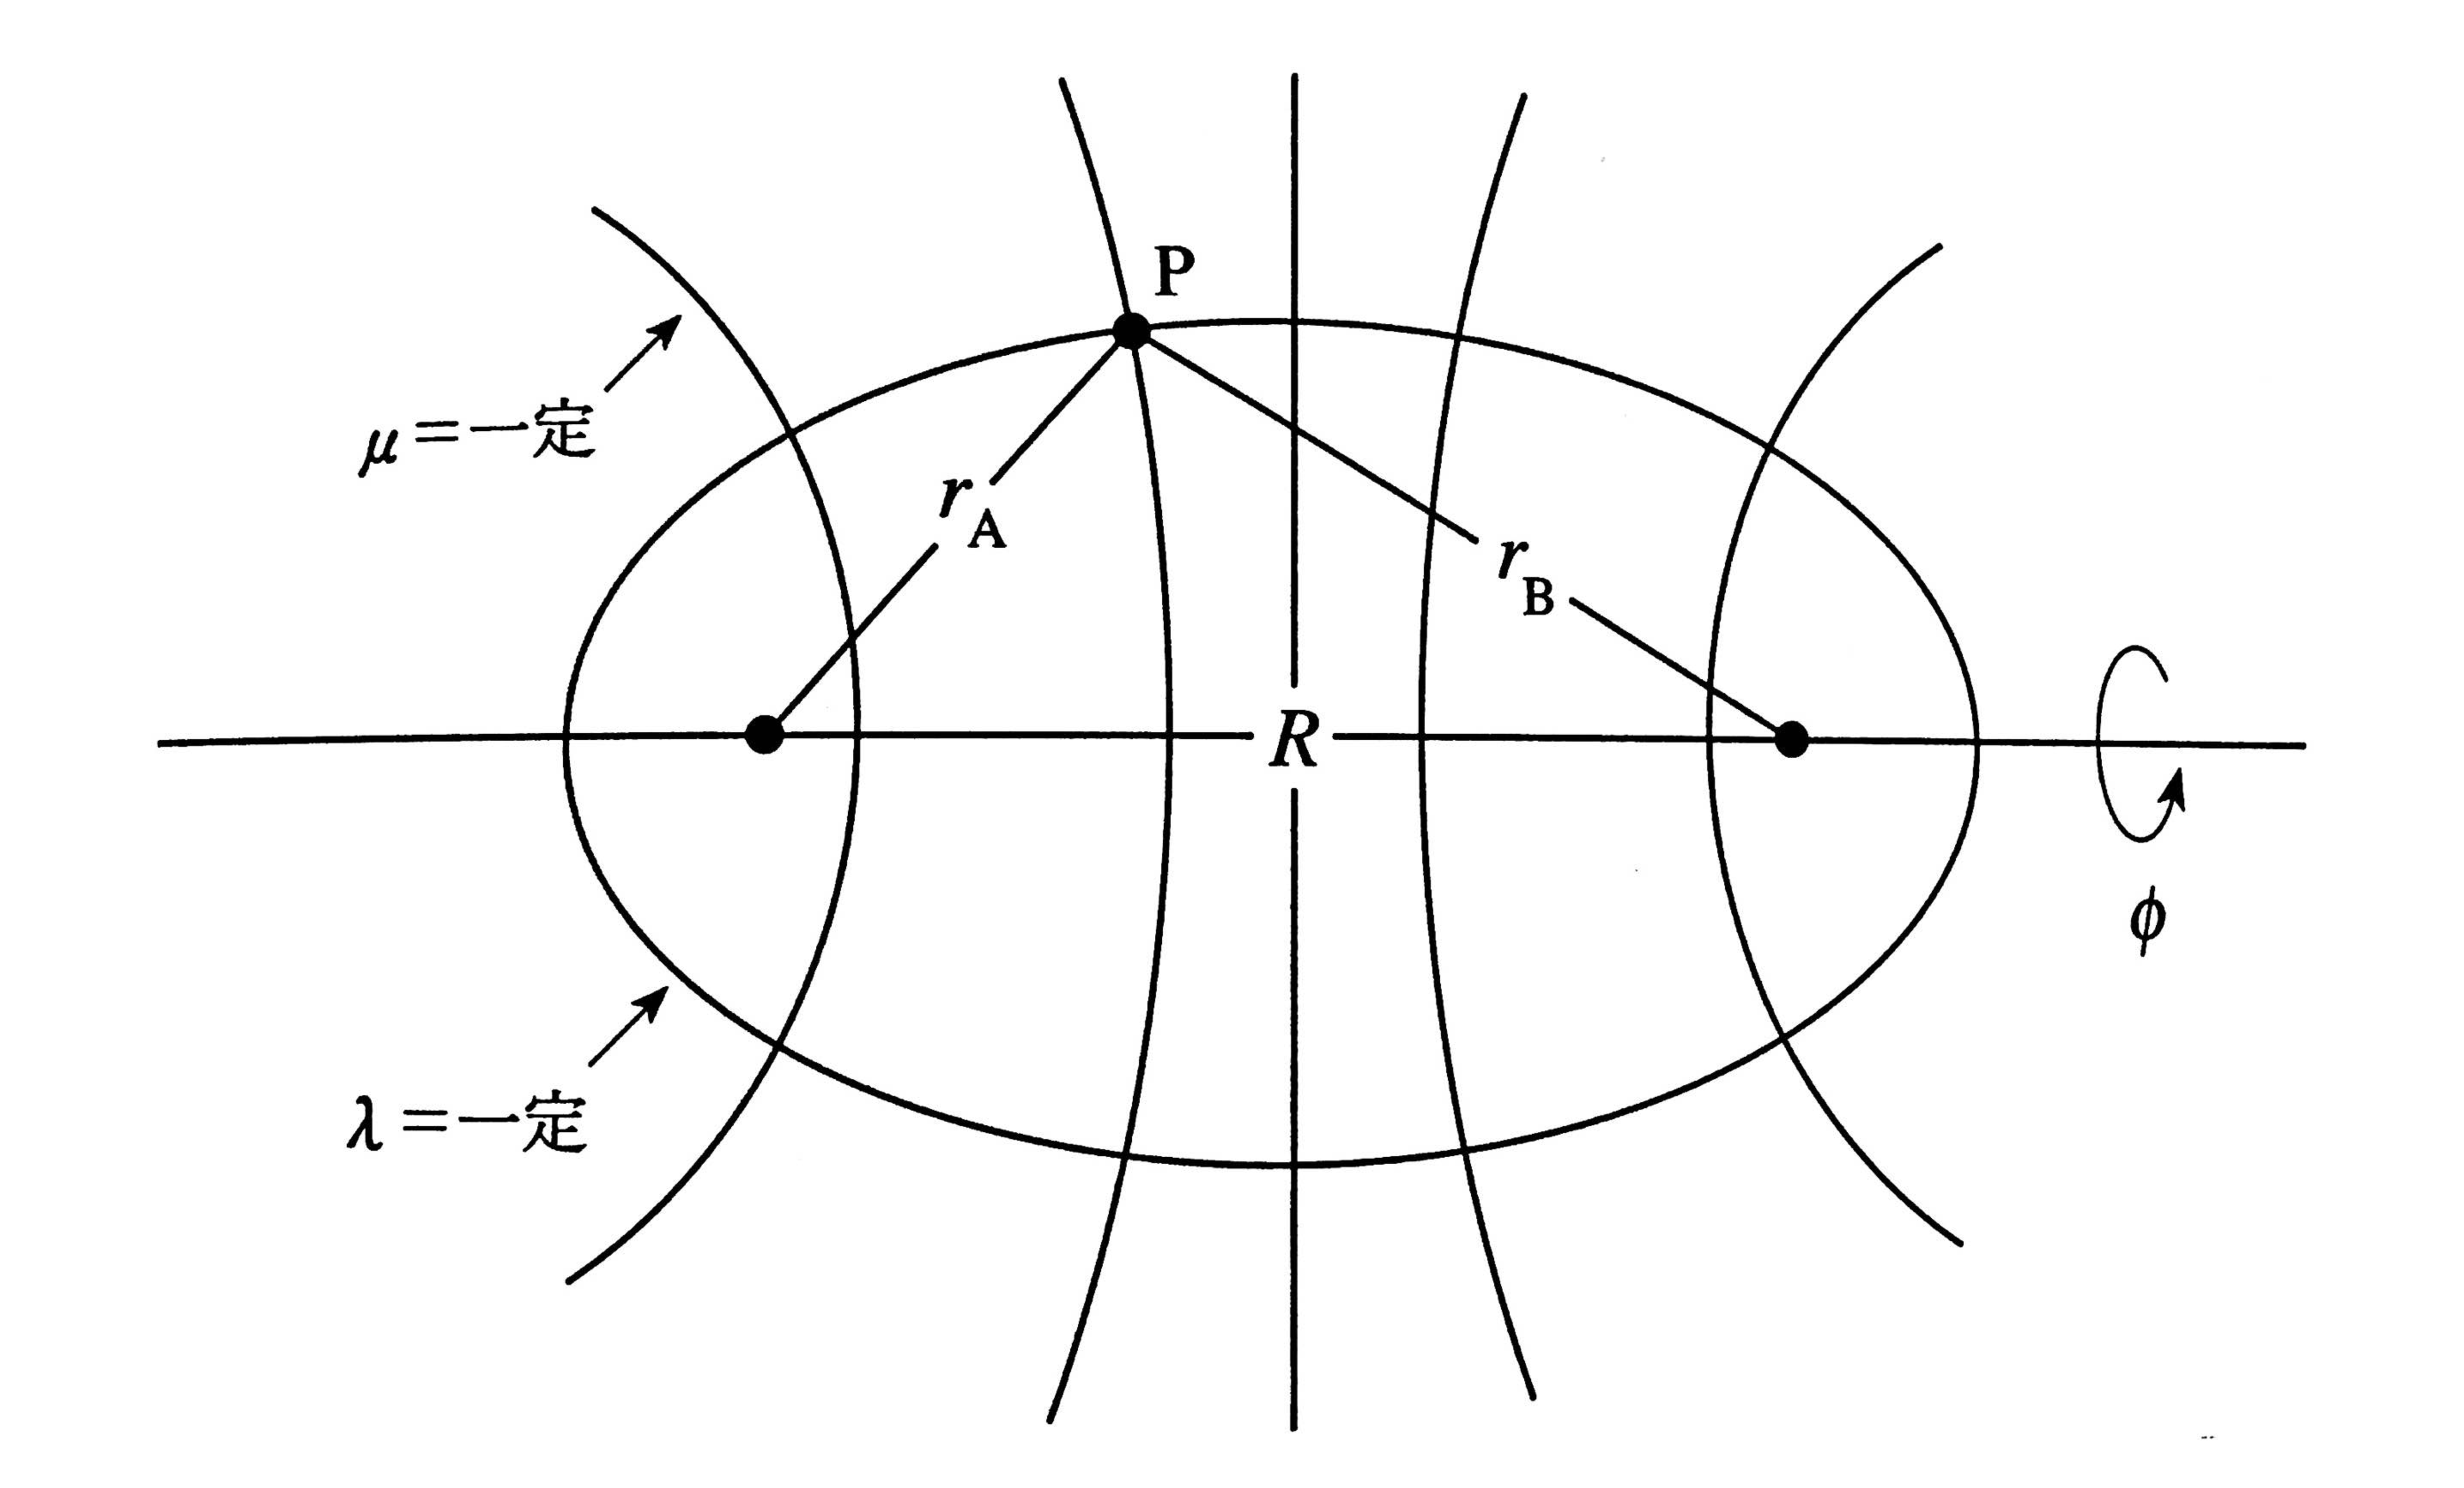
\includegraphics{elliptic.pdf}}
    %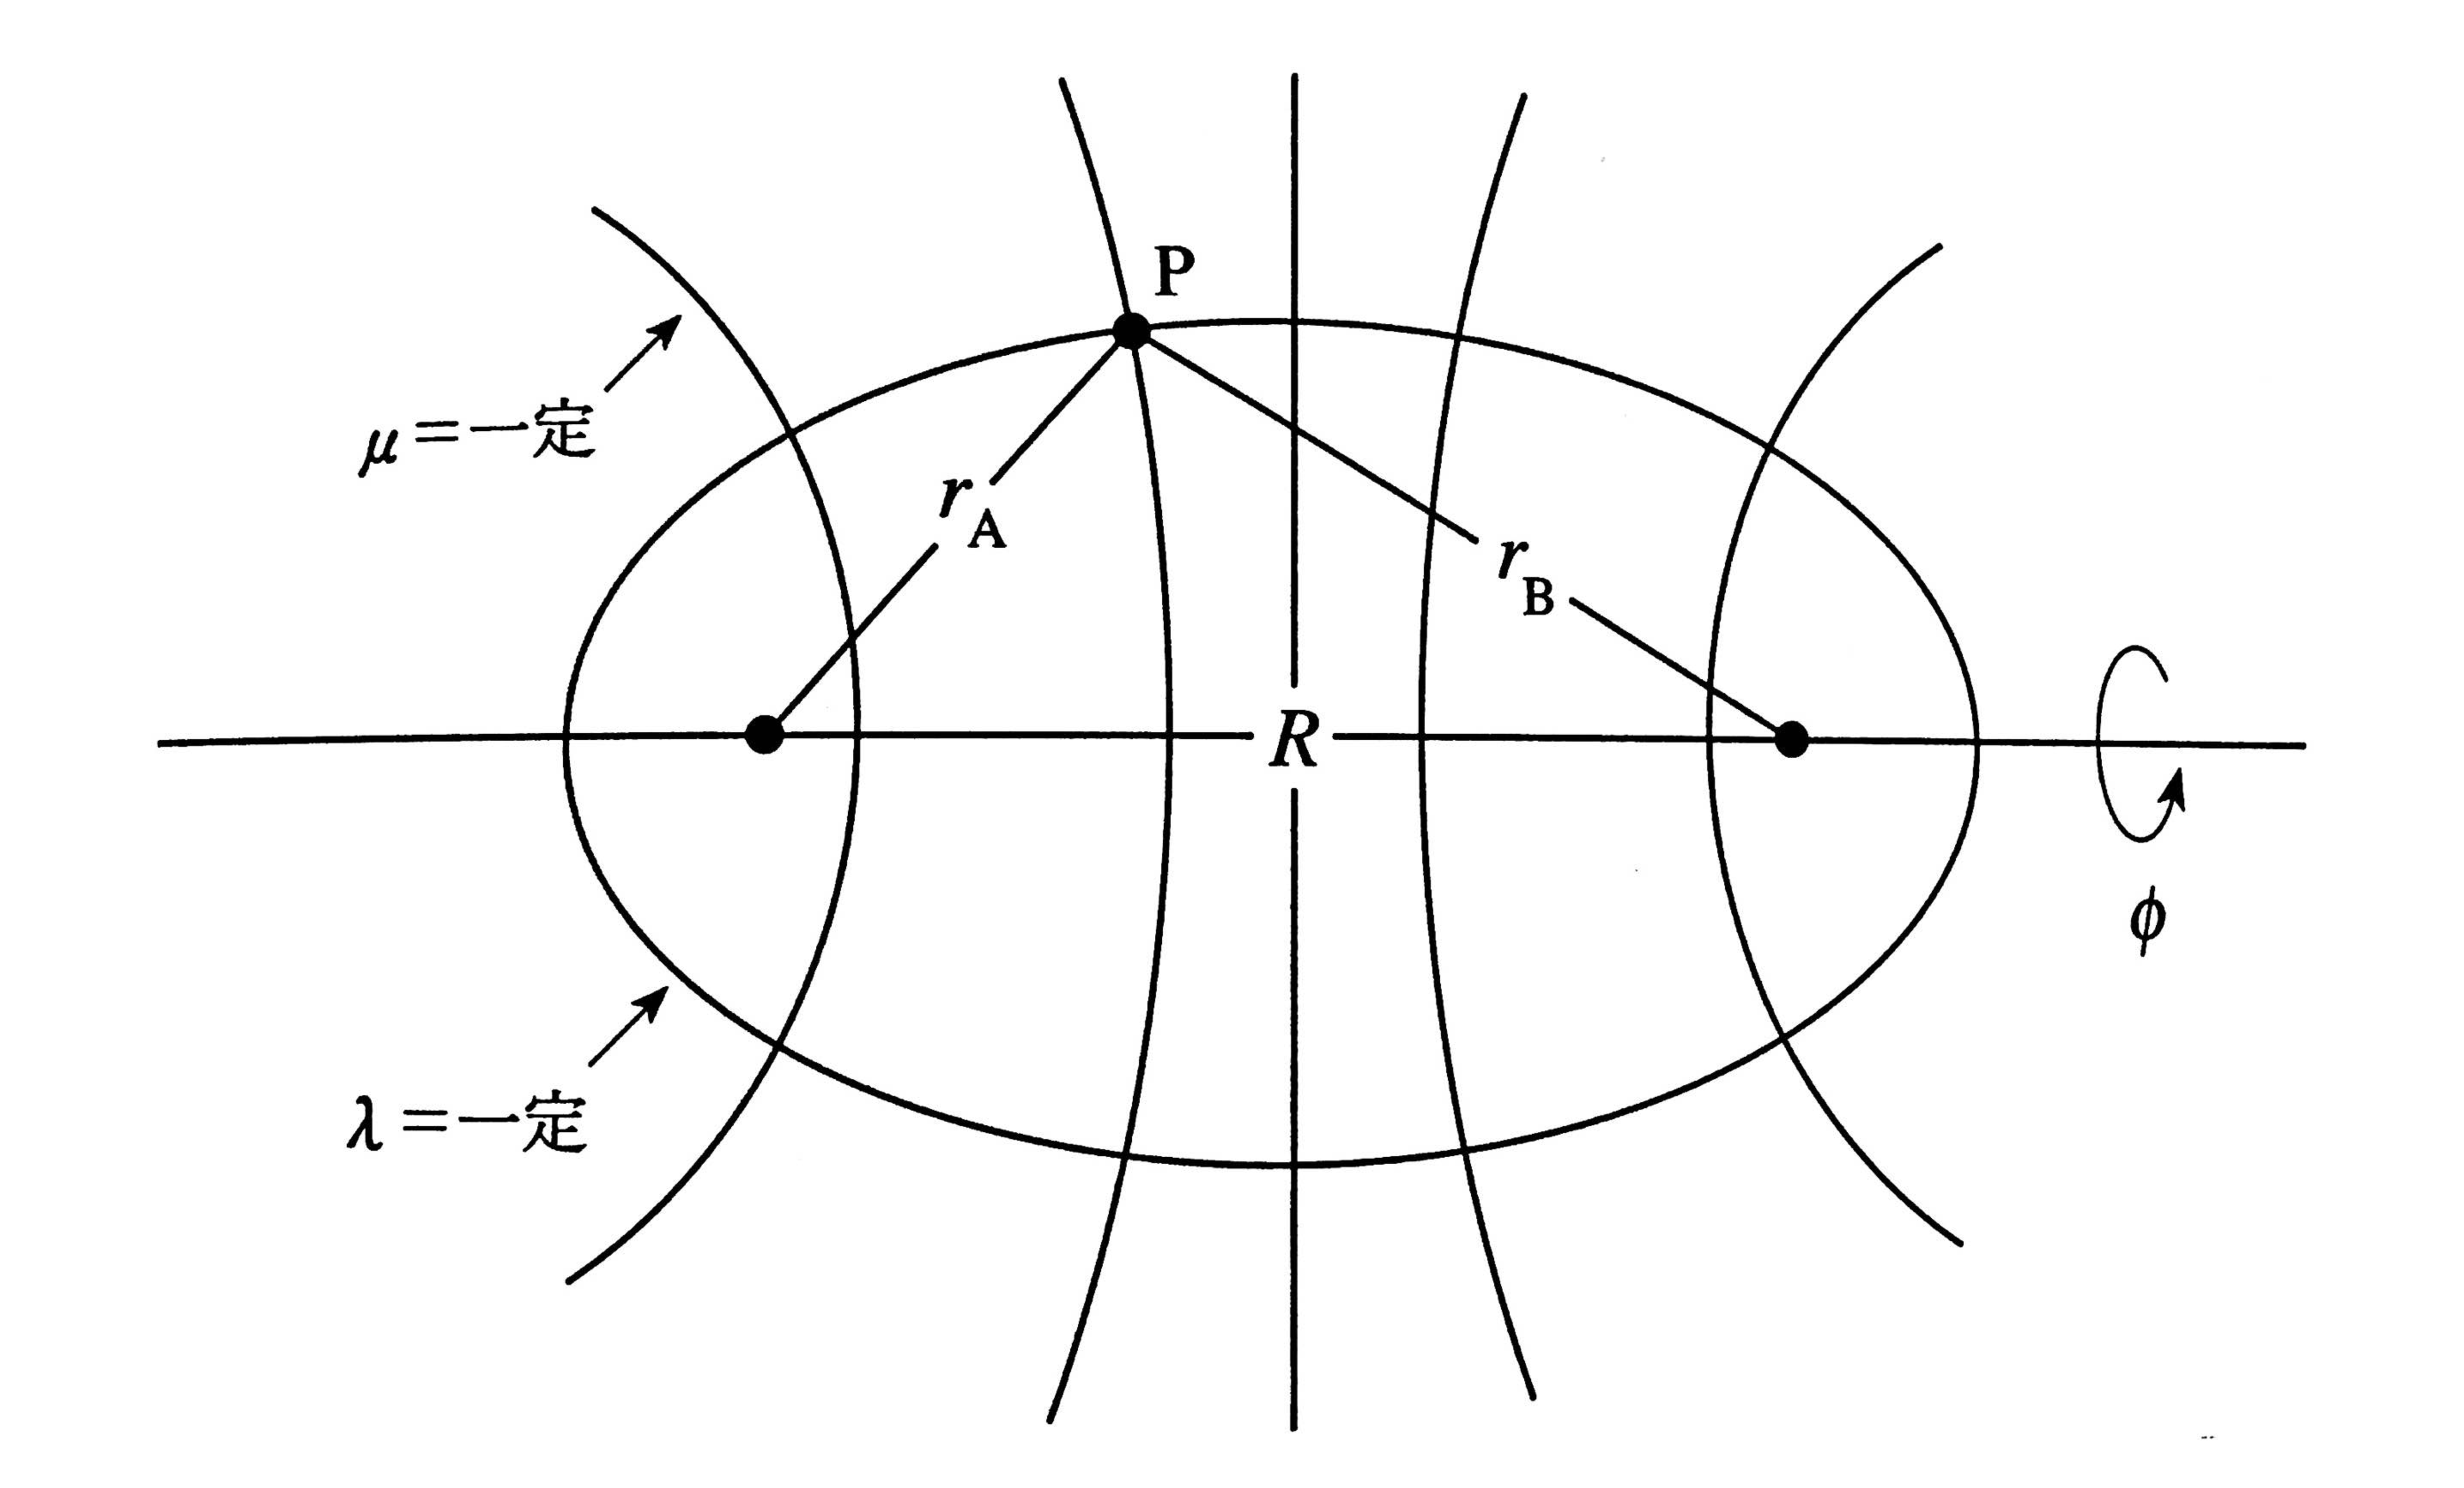
\includegraphics[scale=0.5]{elliptic.pdf}
    \caption{\label{fig:elliptic}
      {
        A volume element in elliptic corrdinate system is given as $d\mathbf{r}=\frac{R^3}{8}(\lambda^2-\mu^2)d\lambda d\mu d\phi$ where $\lambda$ and $\mu$ are defined as $\lambda=\frac{r_A+r_B}{R}$ and $\mu=\frac{r_A-r_B}{R}$. The integration ranges for $\lambda$, $\mu$ and $\phi$ are $1\leq \lambda<\infty$, $-1\leq\mu\leq 1$ and $0\leq\phi\leq 2\pi$, respectively.
      }
    }
    \end{center}
  \end{figure}
}

\noindent
{\bf 解答4}
楕円体座標では
\begin{align}
  S(R)&=\frac{1}{\pi}=\int_1^\infty d\lambda\int_{-1}^{1} d\mu\int^{2\pi}_0d \phi  \ \frac{R^3}{8}(\lambda^2-\mu^2)\exp(-R\lambda)  \nonumber \\
  &=\frac{R^3}{4}\int_1^\infty d\lambda\exp(-R\lambda)\int_{-1}^{1} d\mu (\lambda^2-\mu^2) \label{eq:sol4-1}
\end{align}
となり、ここで上式右辺第二因子は
\begin{align}
  \int_{-1}^{1} d\mu (\lambda^2-\mu^2) = 2\lambda^2-\frac{2}{3}
\end{align}
となる。故に
\begin{align}
  S(R)=\frac{R^3}{2} \int_1^\infty d\lambda \ \left(\lambda^2-\frac{1}{3}\right) \exp(-R\lambda) \label{eq:sol4-2}
\end{align}
を得る。ここで公式を用いて
\begin{align}
  I(\lambda)\equiv\int d\lambda \ \lambda^2 \exp(-R\lambda) = -\exp(-R\lambda)\left(\frac{\lambda^2}{R}+\frac{2\lambda}{R^2}+\frac{2}{R^3}\right)
\end{align}
となる。ここで式(\ref{eq:sol4-2})の$\lambda^2$を含む積分計算には$I(\infty)$が必要となる。これは不定形の極限であり
\begin{align}
  &I(\infty)=0 \\
  &I(1)=-\exp(-R)\left(\frac{1}{R}+\frac{2}{R^2}+\frac{2}{R^3}\right)
\end{align}  
となる。故に
\begin{align}
  \int_1^\infty d\lambda \ \lambda^2 \exp(-R\lambda)=I(\infty)-I(1)=-I(1)=\exp(-R)\left(\frac{1}{R}+\frac{2}{R^2}+\frac{2}{R^3}\right)
\end{align}
となる。式(\ref{eq:sol4-2})は最終的には
\begin{align}
  S(R)&=\frac{R^3}{2}\left[\exp(-R)\left(\frac{1}{R}+\frac{2}{R^2}+\frac{2}{R^3}\right) - \frac{\exp(-R)}{3R}\right] \nonumber \\
  &=\exp(-R)\left(\frac{R^2}{3}+R+1\right)
\end{align}
となる。

\noindent
    {\bf 問題B.} 炭化水素化合物の$\pi$対称性を持つ分子軌道を単純H\"uckel法で計算する。単純H\"ckelモデルでは、$i$番目の$\pi$あるいは$\pi^*$分子軌道は、その分子を構成する$2p_z$軌道の線型結合で近似される。
\begin{align}
  |\psi_\pi^i\rangle=\sum_A^\text{Atoms}C^i_{2p_z\text{A}}|\psi_{2p_z\text{A}}\rangle \label{eq:hueckel}
\end{align}
式(\ref{eq:hueckel})における$C$-係数は変分的に決定される。単純H\"uckelモデルでは、以下の大胆な近似を導入する:
\begin{itemize}
\item Hamiltonian行列の対角要素 ($\langle\psi_{2p_z\text{A}}|H|\psi_{2p_z\text{A}}\rangle$) を単一の定数$\alpha$として近似。
\item 隣り合う原子上の$2p_z$軌道間のHamiltonian行列要素 ($\langle\psi_{2p_z\text{A}}|H|\psi_{2p_z\text{A+1}}\rangle$) を単一の定数$\beta$として近似。
\item 上記以外のHamiltonian行列要素は全て0とする。
\item $2p_z$軌道間の重なり行列は単位行列とする。
\end{itemize}

\noindent
{\bf 問い6} ベンゼンの$\pi$及び$\pi^*$軌道関数及び軌道エネルギーを求めよ。

\noindent
{\bf 解答6}
解くべき永年方程式は
\begin{align}
  \det{|\mathbf{H}-E\mathbf{1}|}=0 \label{eq:secular}
\end{align}
となり、ここでHamiltonian行列は
\begin{align}
  \mathbf{H}=
  \begin{pmatrix}
    \alpha & \beta & 0 & 0 & 0 & \beta \\
    \beta & \alpha & \beta & 0 & 0 & 0 \\
    0 & \beta & \alpha & \beta & 0 & 0 \\
    0 & 0 & \beta & \alpha & \beta & 0 \\
    0 & 0 & 0 & \beta & \alpha & \beta \\
    \beta & 0 & 0 & 0 & \beta & \alpha \\                    
  \end{pmatrix}  
\end{align}
である。$x=\alpha-E/\beta$とすれば、式(\ref{eq:secular})は
\begin{align}
  \det{|\mathbf{H}-E\mathbf{1}|}=
  \beta^6\det
  \begin{vmatrix}
    x & 1 & 0 & 0 & 0 & 1 \\
    1 & x & 1 & 0 & 0 & 0 \\
    0 & 1 & x & 1 & 0 & 0 \\
    0 & 0 & 1 & x & 1 & 0 \\
    0 & 0 & 0 & 1 & x & 1 \\
    1 & 0 & 0 & 0 & 1 & x \\                        
  \end{vmatrix}
  =0\label{eq:secular2}
\end{align}
となる。$\beta\neq0$なので、行列式の性質を用いて、$\det|\cdots|=0$を解く。行列式の値は、ある行(列)に、別の行の定数倍を加えても不変である。式(\ref{eq:secular2})を満たす$x$を決定するストラテジーとして、第一行要素の$x$の次数がもっとも低い行の定数倍をそれ以外の行に加えて、第一列を単位行ベクトルにする。その後余因子展開を行い、行列式のランクを2次にまで落とす。なお6次方程式は、2次方程式の場合のような「代数的な」解の公式が存在しない為、一般に手計算で解析解を得るのは難しい。
\begin{align}
  \begin{vmatrix}
    x & 1 & 0 & 0 & 0 & 1 \\
    1 & x & 1 & 0 & 0 & 0 \\
    0 & 1 & x & 1 & 0 & 0 \\
    0 & 0 & 1 & x & 1 & 0 \\
    0 & 0 & 0 & 1 & x & 1 \\
    1 & 0 & 0 & 0 & 1 & x \\                        
  \end{vmatrix}
  &=
  \begin{vmatrix}
    0 & 1 & 0 & 0 & -x & 1-x^2 \\
    0 & x & 1 & 0 & -1 & -x \\
    0 & 1 & x & 1 & 0 & 0 \\
    0 & 0 & 1 & x & 1 & 0 \\
    0 & 0 & 0 & 1 & x & 1 \\
    1 & 0 & 0 & 0 & 1 & x \\                        
  \end{vmatrix}
  =(-1)^{1+6}\cdot 1\cdot
  \begin{vmatrix}
    1 & 0 & 0 & -x & 1-x^2 \\
    x & 1 & 0 & -1 & -x \\
    1 & x & 1 & 0 & 0 \\
    0 & 1 & x & 1 & 0 \\
    0 & 0 & 1 & x & 1 \\
  \end{vmatrix} \nonumber \\
  &=
  =-
  \begin{vmatrix}
    1 & 0 & 0 & -x & 1-x^2 \\
    x & 1 & 0 & -1 & -x \\
    1 & x & 1 & 0 & 0 \\
    0 & 1 & x & 1 & 0 \\
    0 & 0 & 1 & x & 1 \\
  \end{vmatrix}
  =-
  \begin{vmatrix}
    1 & 0 & 0 & -x & 1-x^2 \\
    0 & 1 & 0 & -1+x^2 & -x-x(1-x^2) \\
    0 & x & 1 & x & -1+x^2 \\
    0 & 1 & x & 1 & 0 \\
    0 & 0 & 1 & x & 1 \\
  \end{vmatrix} \nonumber \\
  &=-
  \begin{vmatrix}
    1 & 0 & -1+x^2 & -2x+x^3 \\
    x & 1 & x & -1+x^2 \\
    1 & x & 1 & 0 \\
    0 & 1 & x & 1 \\
  \end{vmatrix}
  =-
  \begin{vmatrix}
    0 & -x & -2+x^2 & -2x+x^3 \\
    0 & 1-x^2 & 0 & -1+x^2 \\
    1 & x & 1 & 0 \\
    0 & 1 & x & 1 \\
  \end{vmatrix} \nonumber \\
  &=-
  \begin{vmatrix}
    -x & -2+x^2 & -2x+x^3 \\
    1-x^2 & 0 & -1+x^2 \\
    1 & x & 1 \\
  \end{vmatrix}
  =-
  \begin{vmatrix}
    0 & -2+2x^2 & -x+x^3 \\
    0 & -x(1-x^2) & -1+x^2-(1-x^2) \\
    1 & x & 1 \\
  \end{vmatrix} \nonumber \\
  &=-
  \begin{vmatrix}
    0 & -2+2x^2 & -x+x^3 \\
    0 & -x(1-x^2) & -1+x^2-(1-x^2) \\
    1 & x & 1 \\
  \end{vmatrix}
  =-
  \begin{vmatrix}
    -2+2x^2 & -x+x^3 \\
    -x+x^3 & -2+2x^2 \\
  \end{vmatrix} \nonumber \\
  &=-(-2+2x^2)^2+(-x+x^3)^2=(x^3-x+2x^2-2)(x^3-x-2x^2+2) \nonumber \\
  &=\left[(x+2)(x+1)(x-1)\right]\left[(x-2)(x+1)(x-1)\right] \label{eq:determinant}
\end{align}
式(\ref{eq:determinant})より、x=$\pm$2, $\pm$1 (重根) となり、エネルギーは
\begin{align}
E_1&=\alpha+2\beta\\
E_2&=\alpha+ \beta\\
E_3&=\alpha+ \beta\\
E_4&=\alpha- \beta\\
E_5&=\alpha- \beta\\  
E_6&=\alpha-2\beta
\end{align}
となる。また固有ベクトルから、$\pi$分子軌道関数は
\begin{align}
  &|\psi_\pi^1\rangle=\frac{1}{\sqrt{6}}(2|\psi_{2p_z\text{1}}\rangle +   2|\psi_{2p_z\text{2}}\rangle +   2|\psi_{2p_z\text{3}}\rangle + 2|\psi_{2p_z\text{4}}\rangle +   2|\psi_{2p_z\text{5}}\rangle +   2|\psi_{2p_z\text{6}}\rangle) \\
  &|\psi_\pi^2\rangle=\frac{1}{\sqrt{4}}(                                 2|\psi_{2p_z\text{2}}\rangle +   2|\psi_{2p_z\text{3}}\rangle                                -   2|\psi_{2p_z\text{5}}\rangle -   2|\psi_{2p_z\text{6}}\rangle) \\
  &|\psi_\pi^3\rangle=\frac{1}{\sqrt{3}}(2|\psi_{2p_z\text{1}}\rangle + 1/2|\psi_{2p_z\text{2}}\rangle - 1/2|\psi_{2p_z\text{3}}\rangle - 2|\psi_{2p_z\text{4}}\rangle - 1/2|\psi_{2p_z\text{5}}\rangle + 1/2|\psi_{2p_z\text{6}}\rangle) \\
  &|\psi_\pi^4\rangle=\frac{1}{\sqrt{4}}(                                 2|\psi_{2p_z\text{2}}\rangle -   2|\psi_{2p_z\text{3}}\rangle                                +   2|\psi_{2p_z\text{5}}\rangle -   2|\psi_{2p_z\text{6}}\rangle) \\
  &|\psi_\pi^5\rangle=\frac{1}{\sqrt{3}}(2|\psi_{2p_z\text{1}}\rangle - 1/2|\psi_{2p_z\text{2}}\rangle - 1/2|\psi_{2p_z\text{3}}\rangle + 2|\psi_{2p_z\text{4}}\rangle - 1/2|\psi_{2p_z\text{5}}\rangle - 1/2|\psi_{2p_z\text{6}}\rangle) \\
  &|\psi_\pi^6\rangle=\frac{1}{\sqrt{6}}(2|\psi_{2p_z\text{1}}\rangle -   2|\psi_{2p_z\text{2}}\rangle +   2|\psi_{2p_z\text{3}}\rangle - 2|\psi_{2p_z\text{4}}\rangle +   2|\psi_{2p_z\text{5}}\rangle -   2|\psi_{2p_z\text{6}}\rangle) 
\end{align}
となる。

\section{さいごに}

誤植を発見した場合や、つじつまが合わない問題があった場合、齋藤までお知らせください。

\end{document}
